% The method, and the one thing that makes it a measurement.
%
% Five stages. The mark above a stage means its decision rules were
% written, reviewed and committed BEFORE the data that stage would be
% judged on existed -- the design (ADR-0053), the posterior recipe
% (PROTOKOL-UP) and the Hera prediction (PROTOKOL-HT/HS). That is the
% difference between a result and a result chosen after the fact.
\documentclass[tikz,border=0pt]{standalone}
% Shared preamble for the README figures.
%
% Palette: arXiv's HTML dark theme, sampled from a live arXiv HTML paper
% (document.documentElement[data-theme="dark"]) rather than guessed:
%
%   page background  rgb(40, 38, 35)    #282623
%   body text        rgb(249,247,247)   #F9F7F7
%   link / accent    rgb(33, 152, 212)  #2198D4
%   muted text       rgb(173,164,164)   #ADA4A4
%   sunken panel     ~                  #1C1A17
%
% Type is Inter, not a LaTeX book face: these figures are read on a web
% page at small size, where Inter's open apertures hold up and Computer
% Modern does not.
%
% Rules of the house:
%   - The figure carries its own background. It is one designed surface.
%   - If a figure needs a paragraph to be understood, it has failed.
%   - Geometry over charting. The results here are geometric statements;
%     draw the geometry, not a plot of it.
\usepackage[T1]{fontenc}
\usepackage[sfdefault]{inter}
\usepackage{tikz}
\usepackage{amsmath}
\usetikzlibrary{arrows.meta,calc,positioning,fit,backgrounds,decorations.pathreplacing}

% Math should not fall back to Computer Modern next to Inter.
\usepackage[italic,eulergreek]{mathastext}

% --- arXiv dark -----------------------------------------------------
\definecolor{canvas}{HTML}{282623}
\definecolor{sunken}{HTML}{1C1A17}
\definecolor{ink}{HTML}{F9F7F7}
\definecolor{muted}{HTML}{ADA4A4}
\definecolor{accent}{HTML}{2198D4}
\definecolor{hush}{HTML}{3A3733}

\tikzset{
  canvasbg/.style={
    show background rectangle,
    background rectangle/.style={fill=canvas, draw=none},
    inner frame sep=0pt,
  },
  lbl/.style={inner sep=0pt, text=ink},
  dim/.style={inner sep=0pt, text=muted},
}


\newcommand{\STEP}{37}

\begin{document}
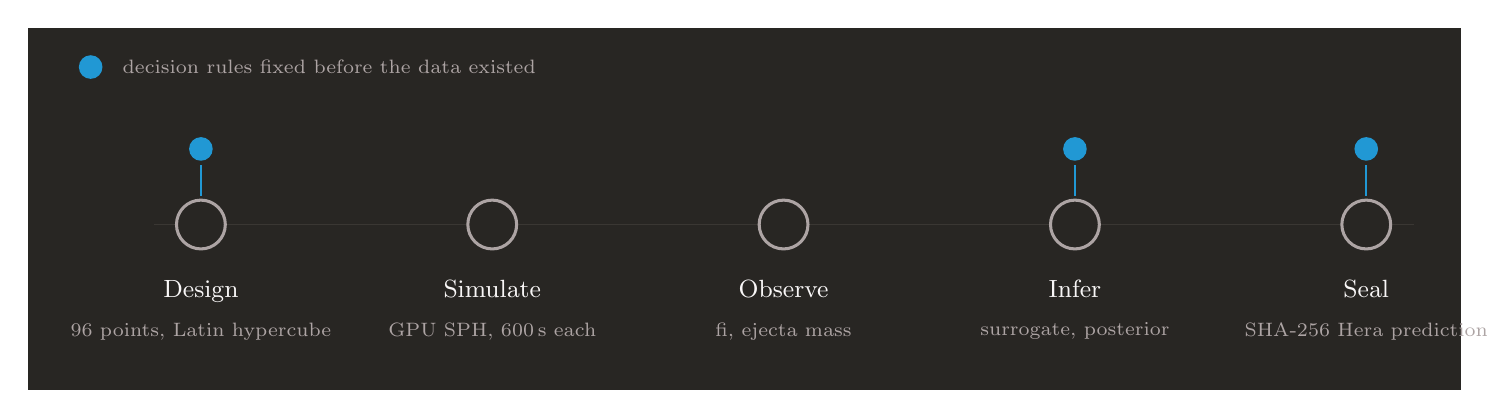
\begin{tikzpicture}[canvasbg, x=1mm, y=1mm]

\useasboundingbox (-22,-21) rectangle (160,25);

% --- the rail -----------------------------------------------------------
\draw[draw=hush, line width=0.7pt] (-6,0) -- (154,0);

% #1 index, #2 name, #3 detail, #4 1 if locked before data
\newcommand{\stage}[4]{%
  \pgfmathsetmacro{\xx}{#1*\STEP}
  \ifnum#4=1
    \draw[draw=accent, line width=0.8pt] (\xx,7.5) -- (\xx,3.6);
    \fill[accent] (\xx,9.6) circle (1.5);
  \fi
  \draw[draw=muted, line width=1.1pt, fill=canvas] (\xx,0) circle (3.1);
  \node[lbl, anchor=north, font=\small] at (\xx,-7) {#2};
  \node[dim, anchor=north, font=\scriptsize, align=center,
        text width=34mm] at (\xx,-12.4) {#3};
}

\stage{0}{Design}{96 points, Latin hypercube}{1}
\stage{1}{Simulate}{GPU SPH, 600\,s each}{0}
\stage{2}{Observe}{$\beta$, ejecta mass}{0}
\stage{3}{Infer}{surrogate, posterior}{1}
\stage{4}{Seal}{SHA-256 Hera prediction}{1}

% --- what the mark means ------------------------------------------------
\fill[accent] (-14,20) circle (1.5);
\node[dim, anchor=west, font=\scriptsize] at (-10,20)
  {decision rules fixed before the data existed};

\end{tikzpicture}
\end{document}
